\begin{lemma}[о четырёх точках]
    $L$ — замкнутая вложенная ломаная. $P, Q, R, S$ — точки ломаной (расположенные именно в таком порядке). $L_1$ — ломаная между $P$ и $R$; $L_2$ — ломаная между $Q$ и $S$; $L_1, L_2$ расположены в одной компоненте связности от $L$; $L_1 \cap L = \{P,R\}, L_2 \cap L = \{S,Q\}$. Тогда $L_1$ и $L_2$ пересекаются.
\end{lemma}
\begin{proof}
    \begin{figure}[htbp]
        \centering
        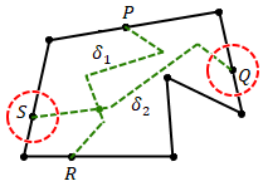
\includegraphics[scale=1]{images/c5.4.png}
        \caption{К лемме о четырёх точках.}
        \label{fig:c5.4}
    \end{figure}

    \begin{figure}[htbp]
        \centering
        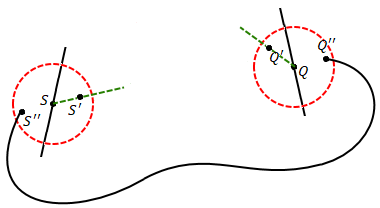
\includegraphics[scale=1]{images/c5.5.png}
        \caption{Выбор точек $S', S'', Q', Q''$.}
        \label{fig:c5.5}
    \end{figure}

    $\tilde{L} = L_1 \cup$ часть ломаной $L$ между $P$ и $R$, содержащая $Q$.
    Рассмотрим точки $S', S'', Q', Q''$ в малых кругах с центрами в $S$ и $Q$ так, как показано на рис.\ref{fig:c5.5} (то есть в разных компонентах, на которые эти круги разбиваются рёбрами ломаной).
    Можно считать, что $S'$ и $Q'$ лежат на $L_2$. Пусть $S'', Q''$ расположены в одной компоненте относительно $L$, которая не содержит $L_1, L_2$.

    Тогда $S'', Q''$ расположены в одной компоненте относительно $\tilde{L}$ (действительно, так как $S'', Q''$ расположены в одной компоненте относительно $L$, значит, их можно соединить какой-то непрерывной кривой, не пересекающей ломаную $L$, причём эта кривая не пересекает и ломаные $L_1, L_2$, поскольку они расположены в другой компоненте. Эта же кривая не пересекает и ломаную $\tilde{L}$, значит, $S'', Q''$ расположены в одной компоненте относительно $\tilde{L}$).

    $Q', Q''$ расположены в разных компонентах относительно $\tilde{L}$ (точки, расположенные по разные стороны от ребра ломаной, лежат в разных компонентах, на которые эта ломаная делит плоскость).

    $S', S''$ расположены в одной компоненте относительно $\tilde{L}$ (очевидно, их можно соединить непрерывной кривой, не пересекающей $\tilde{L}$).

    Суммируя эти утверждения, получаем, что $S', Q'$ расположены в разных компонентах относительно $\tilde{L}$.

    Итак, $S', Q'$ расположены в разных компонентах относительно $\tilde{L}$ и соединены ломаной $\tilde{L_2}$ (полученной из ломаной $L_2$ выбрасыванием маленьких отрезков $SS'$ и $QQ'$, то есть, ломаная $\tilde{L_2}$ не пересекается с ломаной $L$).

    Значит, $\tilde{L_2}$ пересекает ломаную $\tilde{L}$, откуда следует, что $\tilde{L_2}$ пересекает ломаную $L_1$. 

    Но если ломаные $\tilde{L_2}, L_1$ пересекаются, то ломаные $L_2$ и $L_1$ тоже пересекаются, т.к. $\tilde{L_2} \in L_2$. Лемма доказана.
\end{proof}

\begin{statement}
    Граф $K_{3,3}$ не планарен.
\end{statement}
\begin{proof}
    \begin{figure}[h]
        \centering
        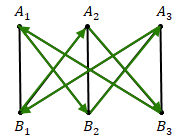
\includegraphics[scale=1]{images/c5.1.png}
        \caption{Граф $K_{3,3}$.}
        \label{fig:c5.1}
    \end{figure}
    \begin{figure}[h]
        \centering
        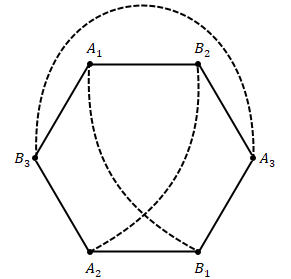
\includegraphics[scale=0.5]{images/c5.2.png}
        \caption{Попытка вложения графа $K_{3,3}$ в плоскость.}
        \label{fig:c5.2}
    \end{figure}
    Предположим, что нам удалось вложить этот граф в плоскость без самопересечений.
    Рассмотрим цикл в графе $A_1B_2A_3B_1A_2B_3A_1$.
    Пусть $K_{3,3}$ вложен в плоскость так, что его рёбра являются ломаными. Тогда этот цикл образует замкнутую ломаную, которая делит плоскость на две компоненты.

    Из оставшихся трёх рёбер $A_1B_1$, $A_2B_2$, $A_3B_3$ по крайней мере два расположены в одной компоненте, причём концы этих рёбер расположены на цикле в нужном порядке (как в лемме о четырёх точках), поэтому они должны пересекаться, откуда следует, что граф $K_{3,3}$ нельзя вложить в плоскость.
\end{proof}

\begin{statement}[Теорема Жордана для замкнутой непрерывной кривой]
    Пусть $L$ — замкнутая вложенная в плоскость кривая. Тогда она разбивает плоскость не менее чем на 2 компоненты.
\end{statement}
\begin{proof}
    Сведём утверждение теоремы к непланарности графа $K_{3,3}$. Будем считать, что на плоскости введены декартовы координаты.
    \begin{figure}[h]
        \centering
        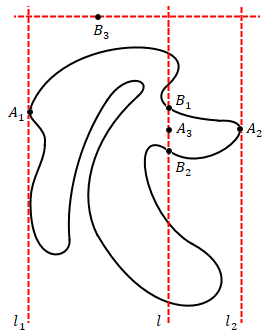
\includegraphics[scale=0.8]{images/c5.3.png}
        \caption{К теореме Жордана.}
        \label{fig:c5.3}
    \end{figure}
    Рассмотрим замкнутую вложенную непрерывную кривую $\gamma$ на плоскости. Пусть $l_1$ и $l_2$ — вертикальные прямые, между которыми расположена кривая $\gamma$ (то есть, $l_1$ и $l_2$ содержат точки кривой, а слева от $l_1$ и справа от $l_2$ точек кривой нет — см.рис.\ref{fig:c5.3}).

    Существование таких прямых следует из свойств непрерывной функции на отрезке: функция $x(t)$ достигает своего минимума и максимума, где \[\gamma(t) = \left(x(t), y(t)\right).\]
    Рассмотрим на прямых $l_1, l_2$ «самые верхние» точки, принадлежащие кривой $\gamma$ (обозначим их $A_1, A_2$, соответственно). Существование таких точек следует из того, что образ кривой $\gamma$ и прямые $l_1, l_2$ — это замкнутые подмножества плоскости, значит, их пересечение тоже будет замкнутым подмножеством плоскости (то есть, супремум этого множества ему принадлежит, поэтому «самые верхние» точки принадлежат прямым $l_1, l_2$).

    Точки $A_1, A_2$ разбивают кривую на две части (условно назовём их верхней и нижней). Проведём ещё одну вертикальную прямую $l$ между прямыми $l_1, l_2$. Из теоремы о промежуточном значении (для функции $x(t)$) следует, что прямая $l$ пересекает кривую $\gamma$. Найдём отрезок $B_1B_2$ на прямой $l$ такой, что:
    \begin{itemize}
        \item $B_1$ лежит на верхней части кривой;
        \item $B_2$ лежит на нижней части кривой;
        \item Между $B_1$ и $B_2$ нет точек кривой.
    \end{itemize}
    Это можно сделать: действительно, из всех точек пересечения $l$ с верхней частью кривой выберем самую нижнюю точку $B_1$, а из всех точек пересечения $l$ с нижней частью кривой, расположенных ниже $B_1$, выберем самую верхнюю точку $B_2$.

    Выберем на отрезке $B_1B_2$ произвольную точку $A_3$ и рассмотрим горизонтальную прямую, расположенную выше, чем кривая $\gamma$ (существование такой прямой следует из того, что функция $y(t)$ ограничена, как непрерывная на отрезке). На этой прямой выберем произвольную точку $B_3$.

    Мы почти получили вложение графа $K_{3,3}$ — точки $A_i$ соединены с $B_j$ (кроме $A_3B_3$), но не соединены между собой. Так как граф $K_{3,3}$ не планарен, то нельзя провести непрерывную кривую, соединяющую $B_3$ и $A_3$, не пересекая уже нарисованных рёбер.

    Рёбра графа $K_{3,3}$, не лежащие на кривой $\gamma$ — это $A_1B_3$ и $B_3A_2$, а также $B_1A_3$ и $A_3B_2$ (составляющие отрезок $B_1B_2$). Допустим, что можно нарисовать кривую $A_3B_3$, не пересекая кривую $\gamma$, тогда она пересекает какую-то из ломаных $A_1B_3A_2$ или $B_1B_2$.

    В этом случае рассмотрим последнюю точку кривой $B_3A_3$, пересекающуюся с $A_1B_3A_2$ и выберем её в качестве $B_3$. Аналогично рассмотрим первую точку пересечения кривой $B_3A_3$ с отрезком $B_1B_2$ и выберем её в качестве $A_3$.

    Тогда кривая, соединяющая новые точки $A_3$ и $B_3$, не будет пересекать ломаные $A_1B_3A_2$, $B_1B_2$ и кривую $\gamma$, что противоречит утверждению о том, что граф $K_{3,3}$ не планарен.

    Значит, $A_3$ и $B_3$ лежат в разных компонентах относительно кривой $\gamma$.
\end{proof}

\subsection{Теорема Эйлера}
\begin{theorem}[Эйлер]
    Пусть дан плоский связный граф $B, P, \Gamma$ — количество вершин, рёбер и частей плоскости, на которые граф разбивает плоскость. Тогда 
    \begin{equation}
        B - P + \Gamma = 2.
        \label{eyler}
    \end{equation}
\end{theorem}